\section{2024年10月21日}
\begin{tcolorbox}[cyan]
    \begin{description}
        \item[\large \textbf{任务}]
        \item[1、] 上次未完成的内容:Polynomial-based Online Planning for Autonomous Drone Racing in Dynamic Environments对比\textbf{2}的提升
        \item[2、] 思考MINCO技术还存在什么缺陷
        \item[3、] 在最初的硕士方向和现在所研究的有什么关系,如果不足以提供支撑,要继续阅读文献
    \end{description}
\end{tcolorbox}
\subsection{Polynomial-based Online Planning for Autonomous Drone Racing in Dynamic Environments(IROS2023)}
\subsubsection{论文主要研究内容}
采用时间均匀MINCO作为轨迹表示形式,对航点作硬约束处理,并结合动态障碍物和大姿态飞行构建了一个重规划框架。\\
(1)\textbf{核心方法}


对于$N$个目标航点,采用$(N+1)$段MICNO轨迹,下述简称为MINCOS轨迹。
其中,$N$个目标航点的位置信息即为MICNOS轨迹中每一段MINCO轨迹的起始或终止点的位置信息。
因此,优化变量即可由单段MINCO轨迹的时间向量和航点和目标航点的速度和加速度向量组成。
经论文Geometrically Constrained Trajectory Optimization for Multicopters 中公式(56、57、63)推导得,
代价函数$\mathcal{W} $对第n段轨迹的起始点$\mathbf{z_{n-1}}$和终止点$\mathbf{z_{n}}$的i阶导数的梯度如下
\begin{equation}
    \frac{\partial \mathcal{W} }{\partial \mathbf{z_{n-1}^{(i)}}} = \mathbf{G_{n0}^T}e_{i} 
\end{equation}
\begin{equation}
\frac{\partial \mathcal{W} }{\partial \mathbf{z_{n}^{(i)}}} = \mathbf{G_{nM}^T}e_{i}
\end{equation}
其中,$e_i$是$\mathbf{I_2s}$的第$i$列。\\
(2)\textbf{实现功能}


    目前实现了对于给定N个航点的的全局路径规划。相比于单段MINCO轨迹优化,对固定航点的速度也进行了优化。
    效果如图\ref{image1}所示。
    \begin{figure}[htbp]
        \centering
        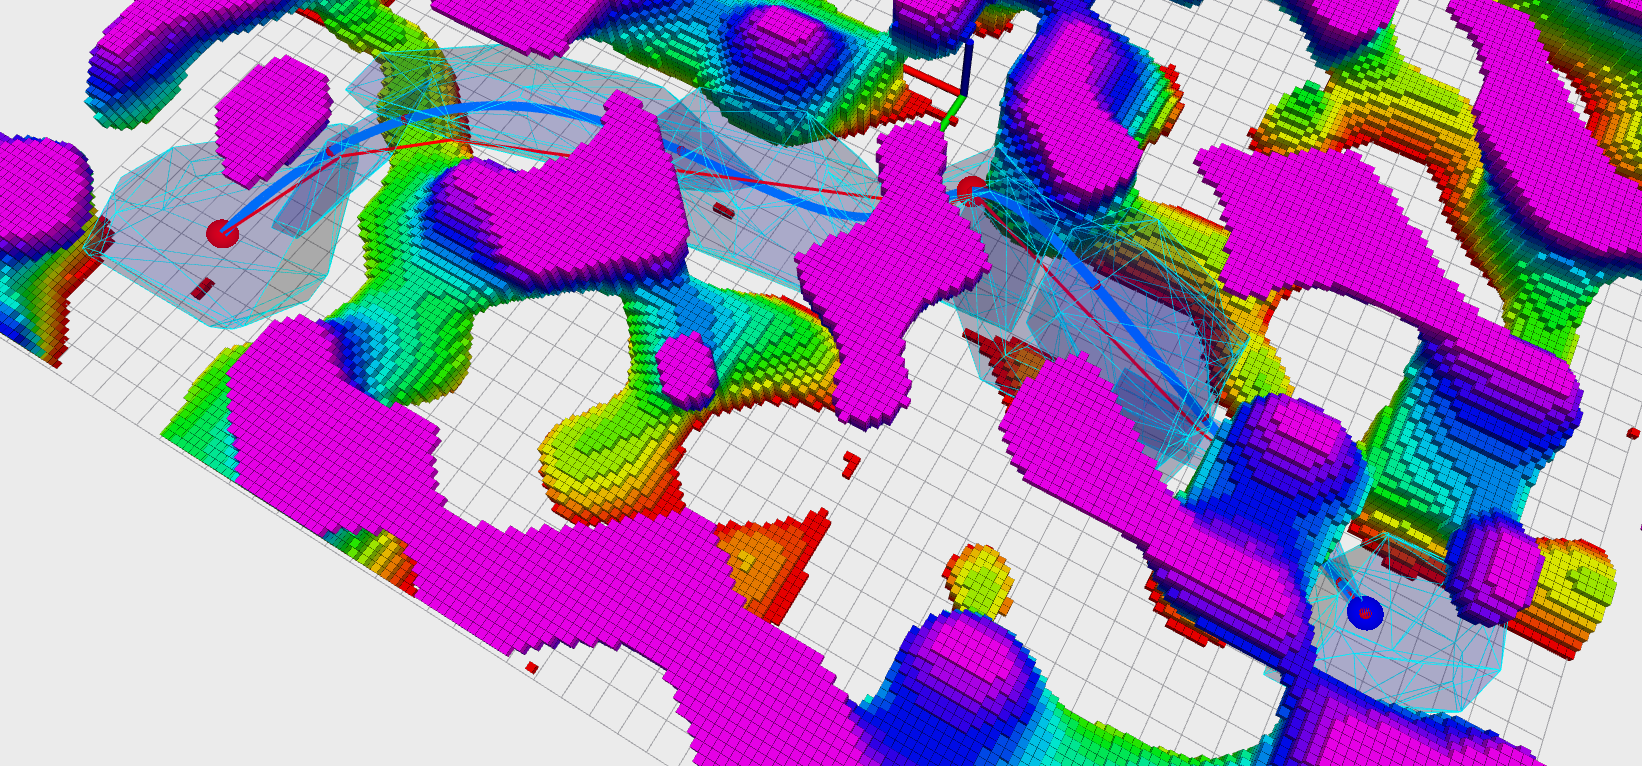
\includegraphics[width=16cm, height=7cm]{image/1.png}
        \caption{航点硬约束的全局路径轨迹效果图}\label{image1}
    \end{figure}\\
(3)\textbf{还未实现功能}


\textbf{钻运动的圈的功能、及多拓扑规划的功能暂未实现}。一方面仿真环境有限,该仿真环境是生成的静态体素地图。
第二,是该仿真是基于全局路径规划的框架,未涉及局部路径规划。\\
(4)\textbf{后续实现方向}


在EGO-PLANNER-V2既存在全局路径规划,又含有局部的路径规划。
不包含动态障碍物但仿真环境更贴近实机,其相比于EGO-PLANNER采用MINCO轨迹,方便代码修改。


尝试对EGO-PLANNER-V2进行修改,并给出一些固定航点接口等。但EGO-PLANNER-V2代码体量大、耦合程度高,存在一定难度。

